%Jennifer Pan, August 2011

\documentclass[10pt,letter]{article}
	% basic article document class
	% use percent signs to make comments to yourself -- they will not show up.

\usepackage{amsmath}
\usepackage{amssymb}
	% packages that allow mathematical formatting

\usepackage{graphicx}
	% package that allows you to include graphics

\usepackage{setspace}
	% package that allows you to change spacing

\onehalfspacing
	% text become 1.5 spaced

\usepackage{fullpage}
	% package that specifies normal margins

\renewcommand{\vector}[1]{\boldsymbol{#1}}
\newcommand{\problem}[1]{\section*{Problem #1}}
\newcommand{\problempart}[1]{\paragraph{#1}}

\begin{document}
	% line of code telling latex that your document is beginning


\title{Problem Set 1}

\author{Nicholas Wu}

\date{Fall 2020}
	% Note: when you omit this command, the current dateis automatically included

\maketitle
	% tells latex to follow your header (e.g., title, author) commands.
\textbf{Note:} I use bold symbols to denote vectors and nonbolded symbols to denote scalars. I primarily use vector notation to shorthand some of the sums, since many of the sums are dot products.

\problem{1}

\problempart{(1)}
The maximization FOCs give us:
 \[ \beta^t c_t^{-\theta} = \lambda_t  \]
 \[ \lambda_t = \lambda_{t+1}(1-\delta + \alpha A k_{t+1}^{\alpha-1})\]
 \[ \beta^t c_t^{-\theta} = \beta^{t+1} c^{-\theta}_{t+1}(1-\delta + \alpha A k_{t+1}^{\alpha-1})\]
 At steady state,
 \[1 = \beta(1-\delta + \alpha A (k^*)^{\alpha-1}) \]
 \[ \beta^{-1} - (1-\delta) = \alpha A (k^*)^{\alpha-1} \]
 \[ \left(\frac{\beta^{-1} - (1-\delta)}{\alpha A}\right)^{1/(\alpha-1)} = k^*\]
 \[ c^* = A(k^*)^\alpha - \delta k^* \]
 \[ c^* = A\left(\frac{\delta}{\alpha A}\right)^{\alpha/(\alpha-1)} - \delta \left(\frac{\delta}{\alpha A}\right)^{1/(\alpha-1)} \]
\problempart{(2)}
See separate file for code.
\problempart{(3)}
Capital is in figure 1, returns in figure 2, wages in figure 3.
\begin{figure}
\centering
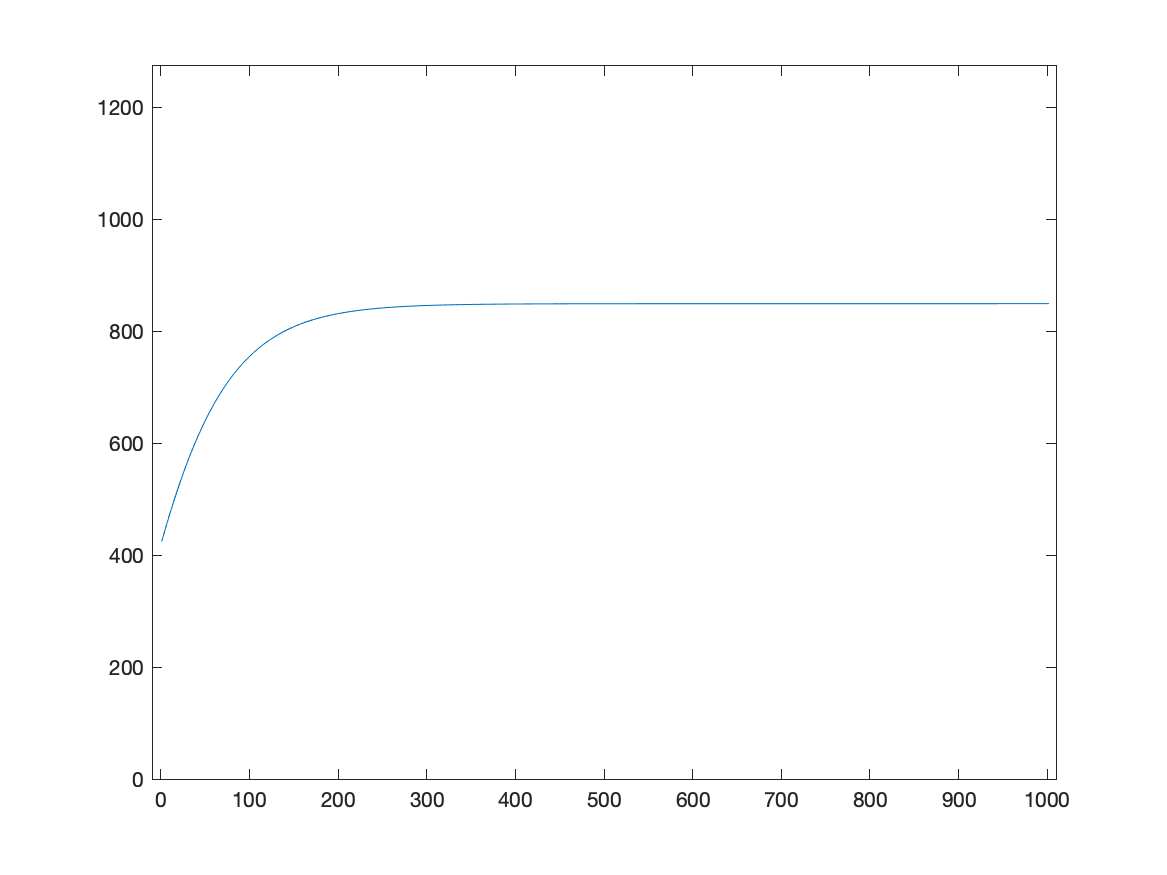
\includegraphics[scale=0.8]{ps1q1fig1}
\caption{Question 1, part 3. Sequence of capital.}
\end{figure}
\begin{figure}
\centering
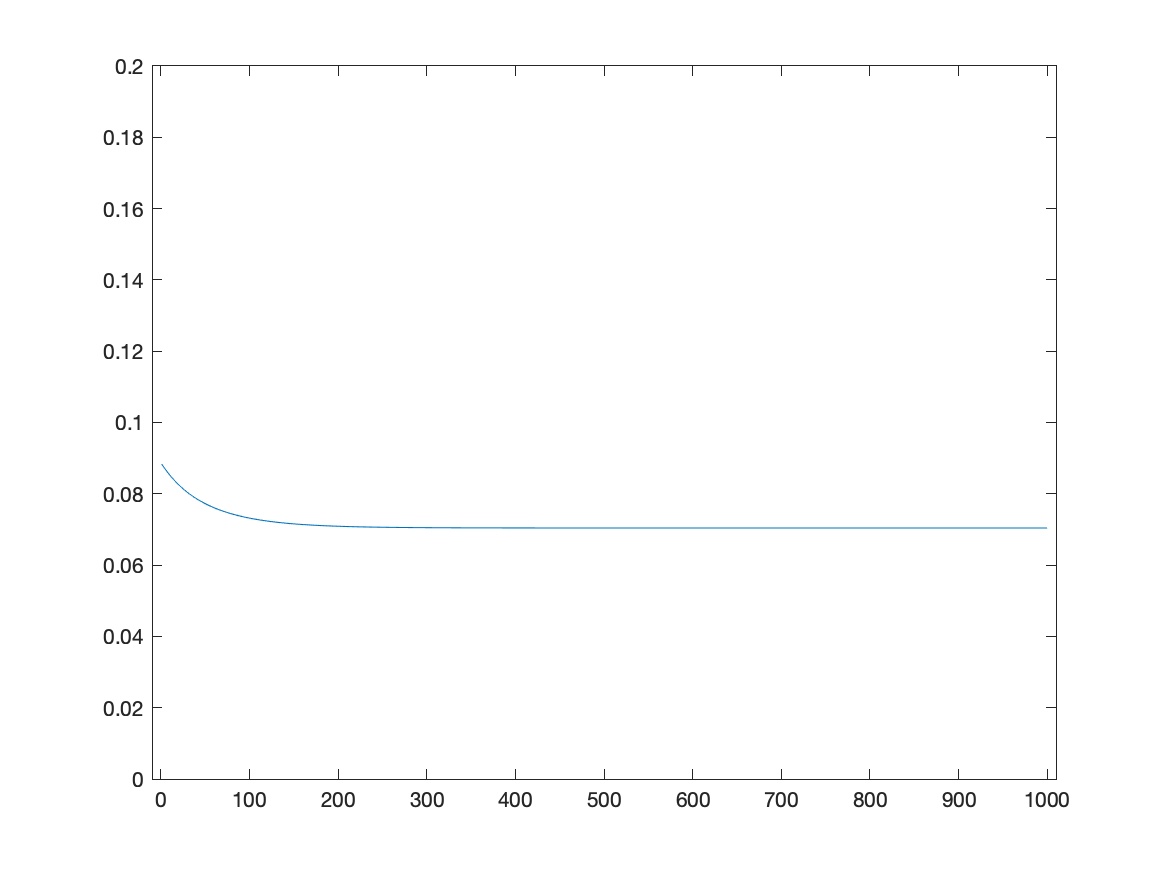
\includegraphics[scale=0.8]{ps1q1fig2}
\caption{Question 1, part 3. Sequence of returns to capital.}
\end{figure}
\begin{figure}
\centering
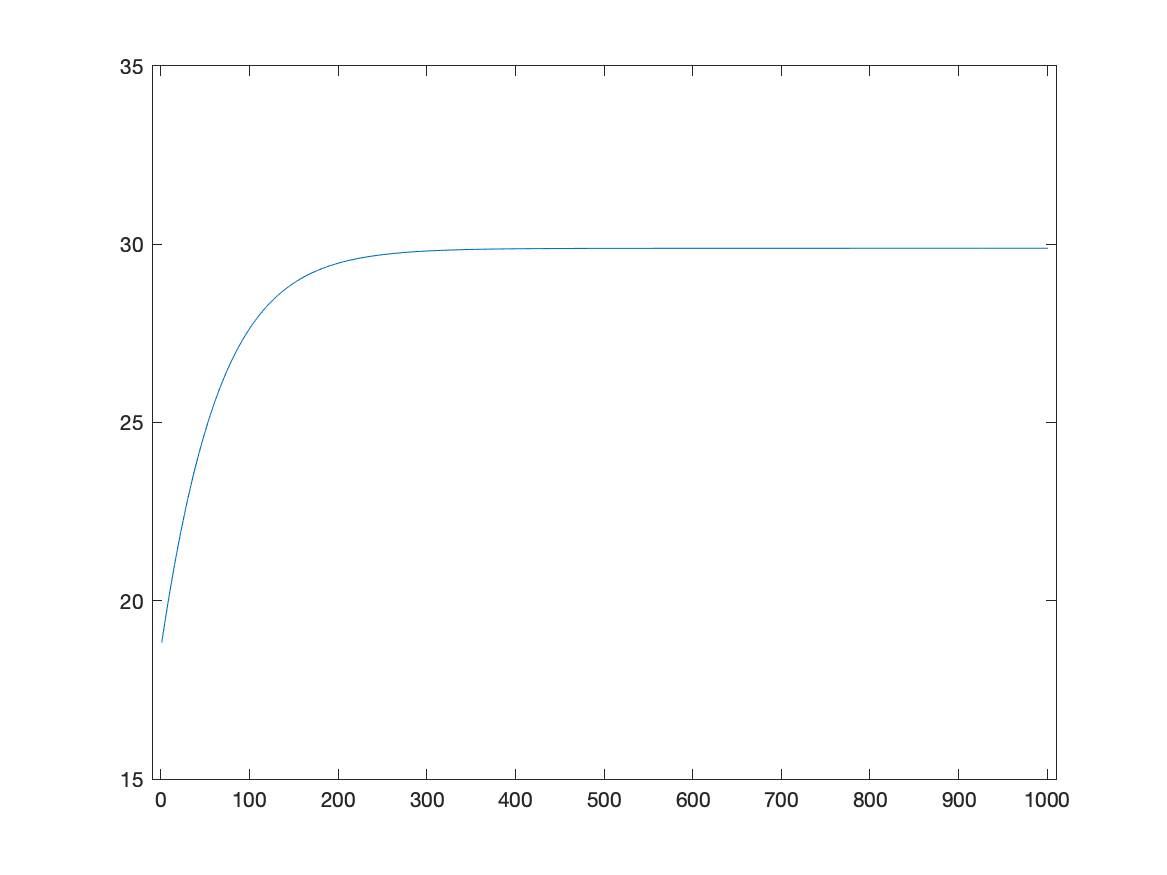
\includegraphics[scale=0.8]{ps1q1fig3}
\caption{Question 1, part 3. Sequence of wages.}
\end{figure}
\problempart{(4)} See figures 4 and 5. As we can see in the graphs, the smaller $\theta$ is, the faster the sequences of capital converge to the new steady state. Increasing $A$ increases net economy production, and hence there will be both an income effect and substitution effect affecting the investment-to-output and consumption-to-output ratios. Since $\theta$ dictates the substitution effect of investment for consumption, the savings rate adjustment depends on $\theta$. When $\theta = 1$, these two effects are equal and in opposite directions, so savings rate remains constant. However, when $\theta < 1$, the substitution effect dominates, so the rate of savings goes down. When $\theta > 1$, the income effect dominates, and the rate of savings increases.
\begin{figure}
\centering
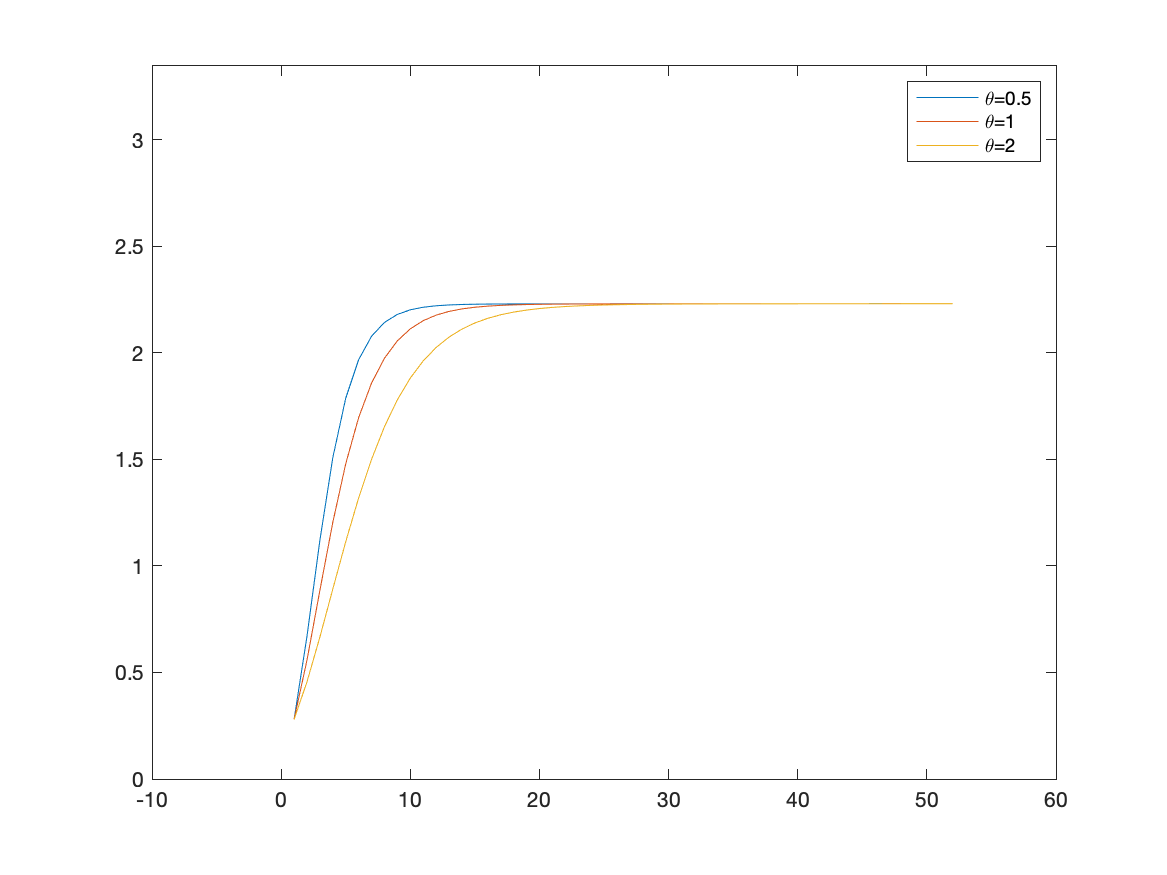
\includegraphics[scale=0.8]{ps1q1fig4}
\caption{Question 1, part 4. Sequence of capital.}
\end{figure}
\begin{figure}
\centering
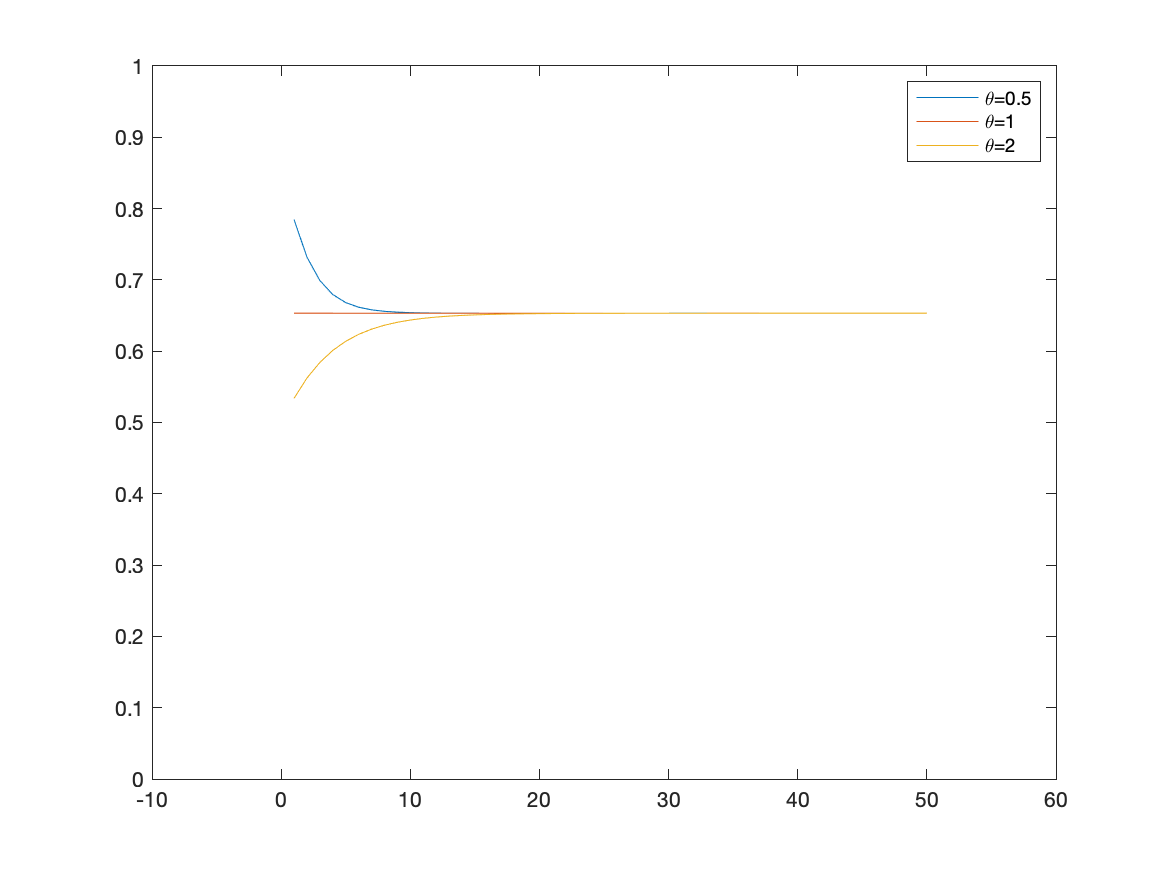
\includegraphics[scale=0.8]{ps1q1fig5}
\caption{Question 1, part 4. Sequence of savings rates.}
\end{figure}


\pagebreak

\problem{2}
Since $\bar{w} > (1-\alpha)(k^*)^\alpha$, the minimum wage is higher than the firms marginal product of labor even at full employment in the steady state. Hence, the minimum wage binds, and is the wage at each time. The employment is then
\[ (1-\alpha)\left(\frac{k_t}{E_t}\right)^\alpha = \bar{w} \]
\[ E_t = k_t \left( \frac{1-\alpha}{\bar{w}} \right)^{1/\alpha}\]
So output is
\[ Y_t = k_t \left( \frac{1-\alpha}{\bar{w}} \right)^{(1-\alpha)/\alpha} \]
And the capital change:
\[ k_{t+1} - k_t = -\delta k_t + s k_t \left( \frac{1-\alpha}{\bar{w}} \right)^{(1-\alpha)/\alpha} \]
\[ k_{t+1} - k_t = \delta k_t \left(\frac{s}{\delta} \left( \frac{1-\alpha}{\bar{w}} \right)^{(1-\alpha)/\alpha} - 1\right) \]
Using the fact that $k = (s/\delta)^{1/(1-\alpha)}$
\[ k_{t+1} - k_t = \delta k_t \left(\left( \frac{(1-\alpha)(k^*)^\alpha}{\bar{w}} \right)^{(1-\alpha)/\alpha} - 1\right) \]
Now, since $(1-\alpha)/\alpha$ is positive and $\bar{w} > (1-\alpha)(k^*)^\alpha$, the parenthesized expression is negative. Further, the rate of decrease is
\[ \rho = \delta\left(\left(1 - \frac{(1-\alpha)(k^*)^\alpha}{\bar{w}} \right)^{(1-\alpha)/\alpha} \right) \]
Hence at every period, $k_{t+1} = (1-\rho) k_t$. Since $\rho$ is independent of $k_t$, we have $k_t \to 0$, which jointly then implies output and employment both drop to 0.
\pagebreak
\problem{3}
\problempart{(1)}
The consumer problem is
\[ \max \sum_{t=0}^\infty \beta^t (\log c_t + g_t) \]
subject to
\[ c_t + i_t \le r_t k_t + w_t \]
\[ k_{t+1} = (1-\tau)i_t + (1-\delta)k_t \]
We can write the Bellman equation:
\[ V(k) = \max_{k'} \left[ \log \left(r k + w - \frac{k' - (1-\delta)k}{1-\tau} \right) + g + \beta V(k') \right] \]
The Euler equation is
\[ \beta ( r_{t+1} + \frac{1-\delta}{1-\tau_{t+1}}) \frac{1}{c_{t+1}} = \frac{1/(1-\tau_t)}{c_t} \]
Letting $f(k) = F(k, 1)$, we have $r_t = f'(k_t)$, so
\[ \beta ( (1-\tau_{t+1})f'(k_{t+1}) + 1-\delta) \frac{1-\tau_t}{1-\tau_{t+1}} = \frac{c_{t+1}}{c_t} \]
\problempart{(2)}
At steady state, we get
\[ \beta ( (1-\bar{\tau})f'(k^*) + 1-\delta) = 1 \]
\[  f'(k^*) = \frac{1 - \beta(1-\delta)}{\beta(1-\bar{\tau})}  \]
\[ i^* = \frac{\delta k^*}{1 - \bar{\tau}}\]
\[ c^* = f(k^*) - i^* \]
\problempart{(3)}
Steady state utility is given by:
\[ \log(c^*) + g^* = \log\left( f(k^*) - \frac{\delta k^*}{1 - \bar{\tau}}\right) + \bar{\tau}\frac{\delta k^*}{1 - \bar{\tau}} \]
Taking the FOC:
\[ \frac{f'(k^*) - \frac{\delta}{1-\bar{\tau}}}{f(k^*) - \frac{\delta k^*}{1 - \bar{\tau}}} + \bar{\tau}\frac{\delta k^*}{1 - \bar{\tau}} = 0 \]
\end{document}
	% line of code telling latex that your document is ending. If you leave this out, you'll get an error
